\chapter{Integrating CCPP with a host model}
\label{chap_hostmodel}
\setlength{\parskip}{12pt}
%\label{section: addhostmodel}
This chapter describes the process of connecting a host model with the pool of CCPP physics schemes through the CCPP framework. This work can be split into several distinct steps outlined in the following sections.

\section{Checking variable requirements on host model side}
\begin{sidewaysfigure}
\begin{lstlisting}[language=Fortran,
                 basicstyle=\scriptsize\ttfamily,
                 label=lst_mandatory_variables_by_ccpp,
                 caption=Mandatory variables that are provided by the CCPP framework (and must not be defined by the host model)]

!! | local_name | standard_name      | long_name                            | units | rank | type      | kind    | intent | optional |
!! |------------|--------------------|--------------------------------------|-------|------|-----------|---------|--------|----------|
!! | errflg     | ccpp_error_flag    | error flag for error handling        | flag  |    0 | integer   |         | none   | F        |
!! | errmsg     | ccpp_error_message | error message for error handling     | none  |    0 | character | len=512 | none   | F        |
!! | loop_cnt   | ccpp_loop_counter  | loop counter for subcycling loops    | index |    0 | integer   |         | none   | F        |
!!
\end{lstlisting}\vskip2ex
\begin{lstlisting}[language=Fortran,
                 basicstyle=\scriptsize\ttfamily,
                 label=lst_mandatory_variables_by_hostmodel,
                 caption=Mandatory variables that must be provided by the host model (local name is not fixed)]

!! | local_name | standard_name      | long_name                            | units | rank | type      | kind    | intent | optional |
!! |------------|--------------------|--------------------------------------|-------|------|-----------|---------|--------|----------|
!! | mpirank    | mpi_rank           | current MPI rank                     | index |    0 | integer   |         | none   | F        |
!! | mpiroot    | mpi_root           | master MPI rank                      | index |    0 | integer   |         | none   | F        |
!! | mpicomm    | mpi_comm           | MPI communicator                     | index |    0 | integer   |         | none   | F        |
!! | mpisize    | mpi_size           | number of MPI tasks in communicator  | count |    0 | integer   |         | none   | F        |
!! | nthreads   | omp_threads        | number of threads for use by physics | count |    0 | integer   |         | none   | F        |
\end{lstlisting}
\end{sidewaysfigure}
The first step consists of making sure that the necessary variables for running the CCPP physics schemes are provided by the host model. A list of all variables required for the current pool of physics can be found in \execout{ccpp\{-,/\}framework/doc/DevelopersGuide/CCPP\_VARIABLES\_XYZ.pdf (\execout{XYZ}: SCM, FV3)}. While most of the variable requirements come from the CCPP physics schemes, a small number of variables are required for correct operation of the CCPP and for compliance with its standards. These variables are described in Listings~\ref{lst_mandatory_variables_by_ccpp} and~\ref{lst_mandatory_variables_by_hostmodel}. In case a required variable (that is not mandatory for CCPP) is not provided by the host model, there are several options:
\begin{itemize}
\item If a particular variable is only required by schemes in the pool that will not get used, these schemes can be commented out in the ccpp prebuild config (see Sect.~\ref{sec_addscheme}).
\item If a variable can be calculated from existing variables in the model, an interstitial scheme (usually called \execsub{scheme\_name\_pre}) can be created that calculates the missing variable. However, the memory for this variable must be allocated on the host model side (i.\,e. the variable must be defined but not initialized in the host model). Another interstitial scheme (usually called \execsub{scheme\_name\_post}) might be required to update variables used by the host model with the results from the new scheme. At present, adding interstitial schemes should be done in cooperation with the GMTB Help Desk (\url{gmtb-help@ucar.edu}).
\item In some cases, the declaration and calculation of the missing variable can be placed entirely inside the host model. Please consult with the GMTB Help Desk.
\end{itemize}

At present, only two types of variable definitions are supported by the CCPP framework:
\begin{itemize}
\item Standard Fortran variables (\execout{character}, \execout{integer}, \execout{logical}, \execout{real}) defined in a module or in the main program. For \execout{character} variables, a fixed length is required. All others can have a \execout{kind} attribute of a kind type defined by the host model.
\item Derived data types (DDTs) defined in a module or the main program. While the use of derived data types as arguments to physics schemes in general is discouraged (see Sect.~\ref{sec_writescheme}), it is perfectly acceptable for the host model to define the variables requested by physics schemes as components of DDTs and pass these components to CCPP by using the correct \execout{local\_name} (see Listing~\ref{lst_metadata_table_hostmodel} for an example).
\end{itemize}
With the CCPP, it is possible to not only refer to components of derived types, but also to slices of arrays in the metadata table as long as these are contiguous in memory (see Listing~\ref{lst_metadata_table_hostmodel} in the following section for an example).

\section{Adding metadata variable tables for the host model}
To establish the link between host model variables and physics scheme variables, the host model must provide metadata tables similar to those presented in Sect.~\ref{sec_writescheme}. The host model can have multiple metadata tables or just one. For each variable required by the pool of CCPP physics schemes, one and only one entry must exist on the host model side. The connection between a variable in the host model and in the physics scheme is made through its \execout{standard\_name}.

The following requirements must be met when defining variables in the host model metadata tables (see also listing~\ref{lst_metadata_table_hostmodel} for examples of host model metadata tables).
\begin{itemize}
\item The \execout{standard\_name} must match that of the target variable in the physics scheme.
\item The type, kind, shape and size of the variable (as defined in the host model Fortran code) must match that of the target variable.
\item The attributes \execout{units}, \execout{rank}, \execout{type} and \execout{kind} in the host model metadata table must match those in the physics scheme table.
\item The attributes \execout{optional} and \execout{intent} must be set to \execout{F} and \execout{none}, respectively.
\item The \execout{local\_name} of the variable must be set to the name the host model cap (see Sect.~\ref{sec_hostmodel_cap}) uses to refer to the variable.
\item The name of the metadata table must match the name of the module or program in which the variable is defined, or the name of the derived data type if the variable is a component of this type.
\item Metadata tables describing module variables must be placed inside the module.
\item Metadata tables describing components of derived data types must be placed immediately before the type definition.
\end{itemize}
\begin{sidewaysfigure}
\begin{lstlisting}[language=Fortran,
                 %basicstyle=\scriptsize\fontfamily{qcr}\fontshape{n}\fontseries{l}\selectfont
                 basicstyle=\scriptsize\ttfamily,
                 label=lst_metadata_table_hostmodel,
                 caption=Example metadata table for a host model]
    module example_vardefs

      implicit none

!> \section arg_table_example_vardefs
!! | local_name | standard_name | long_name | units | rank | type      | kind   | intent | optional |
!! |------------|---------------|-----------|-------|------|-----------|--------|--------|----------|
!! | ex_int     | example_int   | ex. int   | none  |    0 | integer   |        | none   | F        |
!! | ex_real1   | example_real1 | ex. real  | m     |    2 | real      | kind=8 | none   | F        |
!! | errmsg     | error_message | err. msg. | none  |    0 | character | len=64 | none   | F        |
!! | errflg     | error_flag    | err. flg. | flag  |    0 | logical   |        | none   | F        |
!!

      integer, parameter           :: r15 = selected_real_kind(15)
      integer                      :: ex_int
      real(kind=8), dimension(:,:) :: ex_real1
      character(len=64)            :: errmsg
      logical                      :: errflg

! Derived data types

!> \section arg_table_example_ddt
!! | local_name | standard_name | long_name | units | rank | type      | kind   | intent | optional |
!! |------------|---------------|-----------|-------|------|-----------|--------|--------|----------|
!! | ext%l      | example_flag  | ex. flag  | flag  |    0 | logical   |        | none   | F        |
!! | ext%r      | example_real3 | ex. real  | kg    |    2 | real      | r15    | none   | F        |
!! | ext%r(:,1) | example_slice | ex. slice | kg    |    1 | real      | r15    | none   | F        |
!!
      type example_ddt
        logical              :: l
        real, dimension(:,:) :: r
      end type example_ddt

      type(example_ddt) :: ext

    end module example_vardefs
\end{lstlisting}
\end{sidewaysfigure}

\section{Writing a host model cap for the CCPP}
\label{sec_hostmodel_cap}
The purpose of the host model cap is to abstract away the communication between the host model and the CCPP physics schemes. While CCPP calls can be placed directly inside the host model code, it is recommended to separate the cap in its own module for clarity and simplicity. The host model cap is responsible for:
\begin{description}
\item[\textbf{Allocating memory for variables needed by physics.}] This is only required if the variables are not allocated by the host model, for example for interstitial variables used exclusively for communication between the physics schemes.
\item[\textbf{Allocating the \execout{cdata} structure.}] The \execout{cdata} structure handles the data exchange between the host model and the physics schemes and must be defined in the host model cap or another suitable location in the host model. The \execout{cdata} variable must be persistent in memory. Note that \execout{cdata} is not restricted to being a scalar but can be a multi-dimensional array, depending on the needs of the host model. For example, a model that uses a 1-dimensional array of blocks for better cache-reuse may require \execout{cdata} to be a 1-dimensional array of the same size. Another example of a multi-dimensional array of \execout{cdata} is in the GMTB SCM, which uses a 1-dimensional \execout{cdata} array for $N$ independent columns.
\item[\textbf{Calling the suite initialization subroutine.}] The suite initialization subroutine takes two arguments, the name of the runtime suite definition file (of type \execout{character}) and the name of the \execout{cdata} variable that must be allocated at this point. \emph{Note.} The suite initialization routine \execout{ccpp\_init} parses the suite definition file and initializes the state of the suite and its schemes. This process must be repeated for every element of a multi-dimensional \execout{cdata}. For performance reasons, it is possible to avoid repeated reads of the suite definition file and to have a single state of the suite shared between the elements of \execout{cdata}. This is a developmental feature and has implications on the physics initialization. Host model developers interested in this feature should contact the GMTB Help Desk (\url{gmtb-help@ucar.edu}).
\item[\textbf{Populating the \execout{cdata} structure.}] Each variable required by the physics schemes must be added to the \execout{cdata} structure -- or to each element of a multi-dimensional \execout{cdata} -- on the host model side. This is an automated task and accomplished by inserting a preprocessor directive
\begin{lstlisting}[language=Fortran]
#include ccpp_modules.inc
\end{lstlisting}
at the top of the cap (before \execout{implicit none}) to load the required modules (e.\,g. module \execout{example\_vardefs} in listing~\ref{lst_metadata_table_hostmodel}), and a second preprocessor directive
\begin{lstlisting}[language=Fortran]
#include ccpp_fields.inc
\end{lstlisting}
after the \execout{cdata} variable and the variables required by the physics schemes are allocated.

\emph{Note.} The CCPP framework supports splitting physics schemes into different sets that are used in different parts of the host model. An example therefore is the separation between slow and fast physics processes for the GFDL microphysics implemented in FV3GFS: while the slow physics are called as part of the usual model physics, the fast physics are integrated in the dynamical core. The separation of physics into different sets is part of the CCPP prebuild configuration (see Sect.~\ref{sec_ccpp_prebuild_config}), which allows to create multiple include files (e.g. \execout{ccpp\_fields\_slow\_physics.inc} and \execout{ccpp\_fields\_fast\_physics.inc} that can be used by different \execout{cdata} structures in different parts of the model). Please contact the GMTB Help Desk (\url{gmtb-help@ucar.edu}) if you would like to use this feature.
\item[\textbf{Providing interfaces to call CCPP for the host model.}] The cap must provide functions or subroutines that can be called at the appropriate places in the host model time integration loop and that internally call \execout{ccpp\_init}, \execout{ccpp\_physics\_init}, \execout{ccpp\_physics\_run}, \execout{ccpp\_physics\_finalize} and \execout{ccpp\_finalize}, and handle any errors returned.
\end{description}
Listing~\ref{lst_host_cap_template} contains a simple template of a host model cap for CCPP, which can also be found in \execout{ccpp/framework/doc/DevelopersGuide/host\_cap\_template.F90}.
\begin{figure}
\lstinputlisting[language=Fortran,
                 %basicstyle=\scriptsize\fontfamily{qcr}\fontshape{n}\fontseries{l}\selectfont
                 basicstyle=\scriptsize\ttfamily,
                 label=lst_host_cap_template,
                 caption=Fortran template for a CCPP host model cap]{./host_cap_template.F90}
\end{figure}\clearpage
\section{Configuring and running the CCPP prebuild script}
\label{sec_ccpp_prebuild_config}
\begin{figure}
\centerline{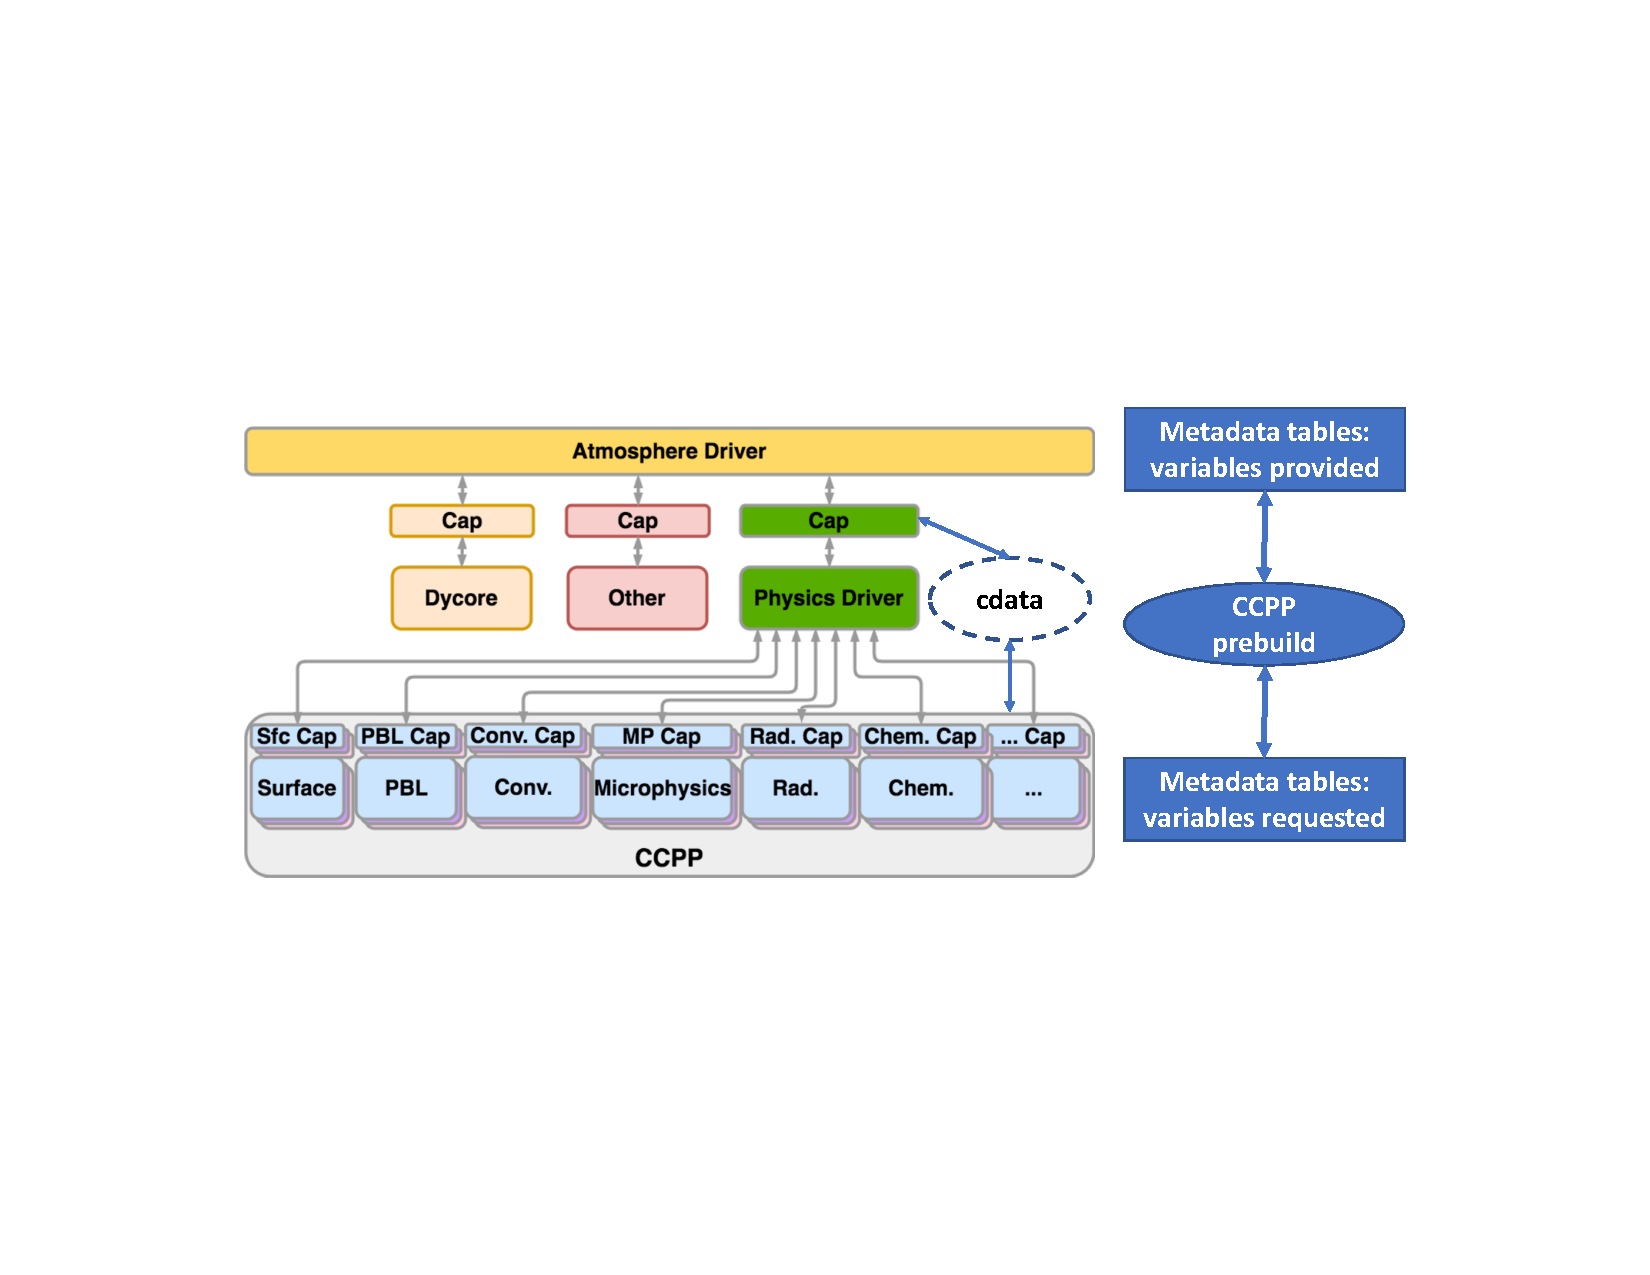
\includegraphics[width=0.85\textwidth]{./images/ccpp_design_with_ccpp_prebuild.pdf}}
\caption{Role of the CCPP prebuild script and the \execout{cdata} structure in the software architecture of an atmospheric modeling system.}\label{fig_ccpp_design_with_ccpp_prebuild}
\end{figure}
The CCPP prebuild script \execout{ccpp/framework/scripts/ccpp\_prebuild.py} is the central piece of code that connects the host model with the CCPP physics schemes (see Figure~\ref{fig_ccpp_design_with_ccpp_prebuild}). This script must be run before compiling the CCPP physics library and the host model cap. The CCPP prebuild script automates several tasks based on the information collected from the metadata tables on the host model side and from the individual physics schemes:
\begin{itemize}
\item Compiles a list of variables required to run all schemes in the CCPP physics pool.
\item Compiles a list of variables provided by the host model.
\item Matches these variables by their \execout{standard\_name}, checks for missing variables and mismatches of their attributes (e.\,g., units, rank, type, kind) and processes information on optional variables (see also Sect.~\ref{sec_writescheme}).
\item Creates Fortran code (\execout{ccpp\_modules.inc}, \execout{ccpp\_fields.inc}) that stores pointers to the host model variables in the \execout{cdata} structure.
\item Auto-generates the caps for the physics schemes.
\item Populates makefiles with schemes and caps.
\end{itemize}

In order to connect the CCPP with a host model \execsub{XYZ}, a Python-based configuration file for this model must be created in the directory \execout{ccpp/framework/scripts}. The easiest way is to copy an existing configuration file in this directory, for example
\begin{lstlisting}[language=bash]
cp ccpp_prebuild_config_SCM.py ccpp_prebuild_config_XYZ.py
\end{lstlisting}
The configuration in \execout{ccpp\_prebuild\_config\_XYZ.py} depends largely on (a) the directory structure of the host model itself, (b) where the \execout{ccpp/framework} and the \execout{ccpp/physics} directories are located relative to the directory structure of the host model, and (c) from which directory the \execout{ccpp\_prebuild.py} script is executed before/during the build process (this is referred to as \execout{basedir} in \execout{ccpp\_prebuild\_config\_XYZ.py}).

Listing~\ref{lst_ccpp_prebuild_config} contains an example for the SCM CCPP prebuild config. Here, it is assumed that both \execout{ccpp/framework} and \execout{ccpp/physics} are located in the top-level directory of the host model, and that \execout{ccpp\_prebuild.py} is executed from the same top-level directory.
\begin{lstlisting}[language=python,
                 basicstyle=\scriptsize\ttfamily,
                 label=lst_ccpp_prebuild_config,
                 float=p,
                 caption=CCPP prebuild config for SCM (shortened)]
# Add all files with metadata tables on the host model side,
# relative to basedir = top-level directory of host model
VARIABLE_DEFINITION_FILES = [
    'scm/src/gmtb_scm_type_defs.f90',
    'scm/src/gmtb_scm_physical_constants.f90'
    ]

# Add all physics scheme dependencies relative to basedir - note that the CCPP
# rules stipulate that dependencies are not shared between the schemes!
SCHEME_FILES_DEPENDENCIES = [] # can be empty

# Add all physics scheme files relative to basedir
SCHEME_FILES = {
    # Relative path : [ list of sets in which scheme may be called ]
    'ccpp/physics/physics/GFS_DCNV_generic.f90' : ['physics'],
    'ccpp/physics/physics/sfc_sice.f'           : ['physics'],
    }

# Auto-generated makefile/cmakefile snippets that contains all schemes
SCHEMES_MAKEFILE = 'ccpp/physics/CCPP_SCHEMES.mk'
SCHEMES_CMAKEFILE = 'ccpp/physics/CCPP_SCHEMES.cmake'

# CCPP host cap in which to insert the ccpp_field_add statements;
# determines the directory to place ccpp_{modules,fields}.inc
TARGET_FILES = [
    'scm/src/gmtb_scm.f90',
    ]

# Auto-generated makefile/cmakefile snippets that contains all caps
CAPS_MAKEFILE = 'ccpp/physics/CCPP_CAPS.mk'
CAPS_CMAKEFILE = 'ccpp/physics/CCPP_CAPS.cmake'

# Directory where to put all auto-generated physics caps
CAPS_DIR = 'ccpp/physics/physics'

# Optional arguments - only required for schemes that use optional arguments.
# ccpp_prebuild.py will throw an exception if it encounters a scheme subroutine
# with optional arguments if no entry is made here. Possible values are:
OPTIONAL_ARGUMENTS = {
    #'subroutine_name_1' : 'all',
    #'subroutine_name_2' : 'none',
    #'subroutine_name_3' : [ 'var1', 'var2'],
    }

# HTML document containing the model-defined CCPP variables
HTML_VARTABLE_FILE = 'ccpp/physics/CCPP_VARIABLES.html'

# LaTeX document containing the provided vs requested CCPP variables
LATEX_VARTABLE_FILE = 'ccpp/framework/doc/DevelopersGuide/CCPP_VARIABLES.tex'

######## Template code to generate include files ########

# Name of the CCPP data structure in the host model cap;
# in the case of SCM, this is a vector with loop index i
CCPP_DATA_STRUCTURE = 'cdata(i)'

# Modules to load for auto-generated ccpp_field_add code
# in the host model cap (e.g. error handling)
MODULE_USE_TEMPLATE_HOST_CAP = \
'''
use ccpp_errors, only: ccpp_error
'''

# Modules to load for auto-generated ccpp_field_get code
# in the physics scheme cap (e.g. derived data types)
MODULE_USE_TEMPLATE_SCHEME_CAP = \
'''
       use machine, only: kind_phys
       use GFS_typedefs, only: GFS_statein_type, ...
'''

# EOF
\end{lstlisting}
\clearpage

Once the configuration in \execout{ccpp\_prebuild\_config\_XYZ.py} is complete, run
\begin{lstlisting}[language=bash]
./ccpp/framework/scripts/ccpp_prebuild.py --model=XYZ [--debug]
\end{lstlisting}
from the top-level directory. Without the debugging flag, the output should look like
\begin{lstlisting}[language=bash,basicstyle=\scriptsize\ttfamily]
INFO: Logging level set to INFO
INFO: Parsing metadata tables for variables provided by host model ...
INFO: Parsed variable definition tables in module gmtb_scm_type_defs
INFO: Parsed variable definition tables in module gmtb_scm_physical_constants
INFO: Parsed variable definition tables in module ccpp_types
INFO: Metadata table for model SCM written to ccpp/physics/CCPP_VARIABLES_SCM.html
INFO: Parsing metadata tables in physics scheme files ...
INFO: Parsed tables in scheme rrtmg_lw
...
INFO: Checking optional arguments in physics schemes ...
INFO: Metadata table for model SCM written to ccpp/framework/doc/DevelopersGuide/CCPP_VARIABLES_SCM.tex
INFO: Comparing metadata for requested and provided variables ...
INFO: Generating module use statements for set physics ...
INFO: Generated module use statements for 4 module(s)
INFO: Generating ccpp_field_add statements for set physics ...
INFO: Generated ccpp_field_add statements for 606 variable(s)
INFO: Generating include files for host model cap scm/src/gmtb_scm.f90 ...
INFO: Generated module-use include file scm/src/ccpp_modules.inc
INFO: Generated fields-add include file scm/src/ccpp_fields.inc
INFO: Generating schemes makefile/cmakefile snippet ...
INFO: Added 81 schemes to ccpp/physics/CCPP_SCHEMES.mk and ccpp/physics/CCPP_SCHEMES.cmake
INFO: Generating caps makefile/cmakefile snippet ...
INFO: Added 64 auto-generated caps to ccpp/physics/CCPP_CAPS.mk and ccpp/physics/CCPP_CAPS.cmake
INFO: CCPP prebuild step completed successfully.
\end{lstlisting}

\section{Building the CCPP framework and physics library}
\label{sec_ccpp_build}
\subsection{Preface}
It is highly recommended to build the CCPP physics library and software framework as part of the host model. Both \execout{ccpp-framework} and \execout{ccpp-physics} use a cmake build system, which can be integrated in the host model's cmake build system, as it is the case for the SCM. For the example of FV3GFS, which employs a traditional make build system, the cmake build for the CCPP framework and physics are triggered by the host model's \execout{compile.sh} script.

\emph{Note.} It is possible to build the CCPP framework standalone, for example for testing purposes. It is generally not possible to build the CCPP physics library without running the CCPP prebuild script, since the build system relies on the auto-generated cmake code snippets that define the physics schemes and caps to compile. Further, any thirdparty libraries required by the physics schemes must be compiled and installed separately and the appropriate compiler and linker flags must be set manually. For example, the CCPP physics used by GMTB's SCM require several of NCEP's libraries (bacio, sp, w3nco); FV3GFS in addition requires the ESMF libraries and, depending on the operating system, also the Intel Math Kernel Library MKL (currently MacOSX only).
\subsection{Standalone ccpp-framework build}\label{sec_ccpp_framework_standalone_build}
The instructions laid out below demonstrate how to build the CCPP framework independently of the host model. It is assumed that the Github repository is checked out into a local directory \execout{ccpp-framework}.
\begin{description}
\item[\textbf{Set environment variables.}] In general, CCPP requires the \execout{CC} and \execout{FC} variables to point to the correct compilers. If threading (OpenMP) will be used inside the CCPP physics or the host model calling the CCPP physics, OpenMP-capable compilers must be used.
\item[\textbf{Build the CCPP framework.}] Use the following steps to build the CCPP framework.
\begin{lstlisting}[language=bash]
cd ccpp-framework
mkdir build && cd build
cmake -DCMAKE_INSTALL_PREFIX=$PWD ..
# add -DOPENMP=ON before .. for OpenMP build
# add -DCMAKE_BUILD_TYPE=Debug before .. for 'Debug' build
make
# add VERBOSE=1 for verbose output
make install
# add VERBOSE=1 after install for verbose output
\end{lstlisting}
\item[\textbf{Update environment variables.}] The previous install step creates directories \execout{include} and \execout{lib} inside the build directory. These directories and the newly built library \execout{libccpp.so} need to be added to the environment variables \execout{FFLAGS} and \execout{LDFLAGS}, respectively (example for bash, assuming the current directory is still the above build directory):
\begin{lstlisting}[language=bash]
export FFLAGS="-I$PWD/include/ccpp $FFLAGS"
export LDFLAGS="-L$PWD/lib -lccpp $LDFLAGS"
\end{lstlisting}
\item[\textbf{Testing the CCPP framework.}] Several unit tests are provided by the CCPP framework. These cover basic functionality and will be expanded to increase the test coverage in future releases. The unit tests are run from the build directory using
\begin{lstlisting}[language=bash]
export LD_LIBRARY_PATH=$PWD/schemes/check/src/check-build:$LD_LIBRARY_PATH
make test
\end{lstlisting}
\end{description}
\subsection{Integration with host model build system}
To allow for a flexible configuration of the CCPP framework and physics with multiple models, the \execout{CMakeLists.txt} configuration files for both packages use a cmake variable \execout{PROJECT}. This variable can be set as part of the cmake call (\execout{cmake -DPROJECT=XYZ}) or by a \execout{CMakeLists.txt} that integrates \execout{ccpp-framework} and \execout{ccpp-physics}. If not specified, \execout{PROJECT} is set to 'Unknown'.

The basic steps to build the CCPP framework and physics for a specific host model are outlined in the following.
\begin{description}
\item[\textbf{Recommended directory structure.}] As mentioned in Section~\ref{sec_ccpp_prebuild_config}, we recommend placing the two repositories \execout{ccpp-framework} and \execout{ccpp-physics} into directories \execout{ccpp/framework} and \execout{ccpp/physics} relative to the top-level directory of the host model, and to adapt the CCPP prebuild config such that it can be run from the top-level directory.
\item[\textbf{Set environment variables.}] In addition to the compiler variables \execout{CC} and \execout{FC}, the CCPP physics require further enviroment variables for thirdparty libraries used by the physics schemes. The setup scripts for SCM (in \execout{scm/etc}) or FV3GFS (in \execout{conf} or \execout{modulefiles}) provide useful examples for the correct environment settings.
\item[\textbf{Build the CCPP framework.}] See previous section on how to build the CCPP framework. The cmake variable \execout{PROJECT} can be set to customize the build using \execout{ccpp/framework/CMakeLists.txt}. This includes preprocessor flags such as \execout{-DMPI}.
\item[\textbf{Update environment variables.}] See previous section on how to update the compiler and linker flags.
\item[\textbf{Build CCPP physics library.}] Before building \execout{ccpp-physics}, its top-level cmake configuration \execout{ccpp/physics/CMakeLists.txt} must be customized for the host model. This includes compiler flags, preprocessor flags etc. The user is referred to the existing configurations. The CCPP physics library is built starting from the build directory \execout{ccpp/framework/build}:
\begin{lstlisting}[language=bash]
cd ../.. # back to top-level directory
cd ccpp/physics
mkdir build && cd build
cmake ..
# add -DOPENMP=ON before .. for OpenMP build
# note that OpenMP build requires finding
# detect_openmp.cmake from ccpp/framework/cmake
make
# add VERBOSE=1 after install for verbose output
\end{lstlisting}
\end{description}
Following these steps, the include files and the library \execout{libccpp.so} that the host model needs to be compiled and linked against are located in \execout{ccpp/framework/build/include} and \execout{ccpp/framework/build/lib}. Note that there is no need to link the host model to the CCPP physics library in \execout{ccpp/physics/build}, as long as it is in the search path of the dynamic loader of the OS (for example by adding the directory \execout{ccpp/physics/build} to the \execout{LD\_LIBRARY\_PATH} environment variable). This is because the CCPP physics library is loaded dynamically by the CCPP framework using the library name specified in the runtime suite definition file (see the GMTB Single Column Model Technical Guide v2.1, Chapter 6.1.3, (\url{https://dtcenter.org/gmtb/users/ccpp/docs/}) for further information). Setting the environment variables \execout{FFLAGS} and \execout{LDFLAGS} as described for the CCPP framework standalone build in Sect.~\ref{sec_ccpp_framework_standalone_build} should be sufficient to compile the host model with its newly created host model cap (Sect.~\ref{sec_hostmodel_cap}) and connect to the CCPP library and framework.

For a complete integration of the CCPP infrastructure and physics library build systems in the host model build system, users are referred to the existing implementations in GMTB SCM and FV3GFS.